\newpage\section{Equipe de Controle}
Considerando o escopo do projeto, o grupo responsável pela parte de controle, associado às informações elaboradas pelos demais grupos apresentará, por meio deste relatório, uma proposta de construção do sistema a partir da utilização de sensores para o monitoramento dos parâmetros: temperatura, pressão, fluxo e nível.\\
Observando as duas propostas apresentadas anteriormente, onde um sensor de temperatura principal seria auxiliado por sensores de temperatura de redundância, tem-se que a proposta definida é semelhante. A diferença está no foco dado à cada sensor em diferentes períodos do teste do foguete híbrido. Durante a realização do teste, os sensores de temperatura internos (localizados no reservatório e na tubulação) serão analisados com maior atenção, a fim de manter a faixa de temperatura no nível de bom funcionamento do sensor de pressão da Kistler. Após o encerramento do teste, o foco principal estará no sensor de temperatura externo (localizado no adaptador da câmara de combustão), já que a transferência de calor que se dá após o teste é alta e deve-se controlar a temperatura do sistema para que os componentes mantenham sua integridade.\\
Diante disso, há no mercado uma gama enorme de sensores que podem ser escolhidos para o funcionamento de um projeto, e a escolha destes deve levar em consideração não só questões operacionais do produto requisitado, mas também uma relação custo-benefício. Além do mais, criticidade do projeto demanda o uso de sub-sistemas redundantes, garantindo maior confiabilidade ao controle do sistema.\\
Portanto, considerando os requisitos necessários para o bom funcionamento do sistema, foram definidos seis sensores, sendo eles três de temperatura, um de pressão, um de fluxo e um de nível, que realizarão o monitoramento dos parâmetros cruciais. Serão utilizados também um microcontrolador, bem como circuitos paralelos de comunicação, amplificação de sinal e alimentação.\\
\section{Desenvolvimento}
O sistema de controle foi baseado em cinco partes, sendo elas: coleta de dados, amplificação de sinais, análise de dados, transferência de dados e controle de resposta.
\subsection{Coleta de Dados}
A parte de coleta de dados será realizada pelos sensores e será a porta de entrada para os dados de monitoramento dos principais parâmetros durante a realização do teste. O sensor de pressão da Kistler estará em funcionamento juntamente com todo o sistema de arrefecimento durante o teste. Sendo assim os principais parâmetros a serem monitorados são temperatura (sensor de pressão da Kistler, tubulação e reservatório), pressão (tubulação), fluxo (tubulação) e nível (reservatório). Portanto, após diversas pesquisas, os modelos mais adequados para cumprirem essas funções foram:
\begin{itemize}
	\item \textbf{Sensor de Temperatura para o adaptador da câmara de combustão}:
	\begin{itemize}
		\item \textbf{ Modelo:} TJ36-CASS-116G-6-CC-XCIB;
		\item \textbf{ Descrição:} Sonda TJ36 com cabo de ligação com isolamento cerâmico de Nextel® e revestimento trançado de Inconel® 600, terminações desencapadas;
		\item \textbf{ Material da Bainha:} sonda em aço inox 304;
		\item \textbf{ Categoria do termopar:} tipo K;
		\item \textbf{ Tipo de Junção:} Aterrada;
		\item \textbf{ Dimensões:}
		\begin{itemize}
			\item  Diâmetro da sonda de 1,59 mm (1/16” pol);
			\item Comprimento de 150 mm (6” pol);
			\item Comprimento do fio de 1,0 m.
		\end{itemize}
		\item \textbf{ Temperatura de operação:} -200 ºC a 899 ºC;
		\item \textbf{ Preço:} R\$382,00.
	\end{itemize}
	
\end{itemize}
\begin{figure}[!htb]                   
	\centering                          
	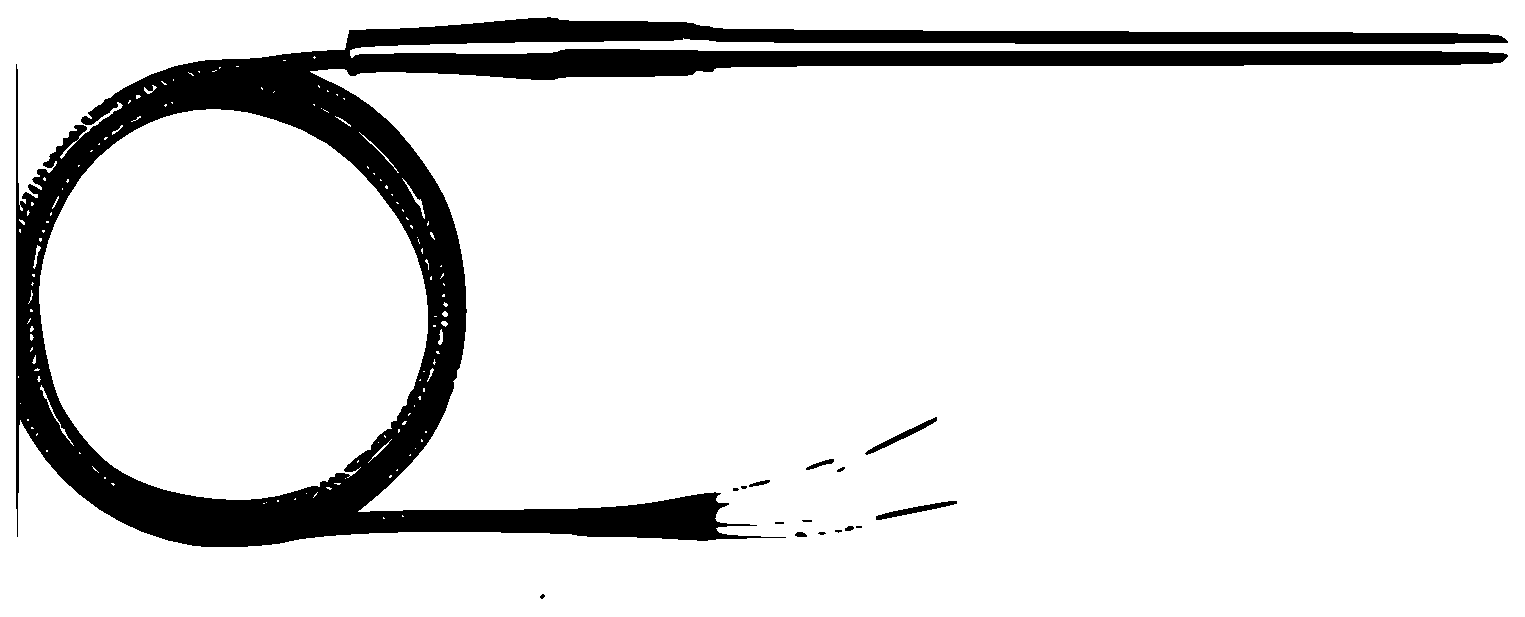
\includegraphics[scale=0.4]{figuras/Sensor1.eps}
	\caption{Sensor de Temperatura para o adaptador da câmara de combustão}               
\end{figure}
\subsection{Explicação:}
	A escolha deste sensor se deve ao fato principalmente da magnitude da temperatura no adaptador que, por meio de simulações realizadas pelo grupo de transmissão de calor, alcança a faixa de até $450^o C$, na posição em que o sensor de pressão principal está localizado. Foi estabelecido um fator de segurança igual a 2, teorizando uma temperatura máxima de $900^{o}C$ no adaptador, o que dá maior margem para erros e falhas. Dessa forma, a escolha de um termopar tipo K se justifica, se for considerado a faixa de medição padrão $(-200^o C a 1250^o C)$ e a alta disponibilidade desse tipo de termopar no mercado.\\
	A junção da bainha é do tipo aterrada, onde os fios do termopar estão em contato físico direto com o interior da parede da sonda. Isso resulta em uma relação resposta/proteção ideal para o caso analisado, já que o material utilizado é o aço, que é conhecidamente um bom condutor térmico. Comparativamente, se fosse utilizada uma junção isolada, o tempo de resposta seria mais demorado, já que entre os fios do termopar e a parede da sonda existe um isolamento que impede o contato direto entre os dois. Já para uma junção exposta o efeito seria o contrário, com um tempo de resposta mais ágil, porém os fios do termopar estariam em maior risco de serem danificados e comprometerem o sensoriamento.\\
	Considerando também o local onde o sensor deverá ser acoplado, as dimensões do produto são apropriadas. Porém, este dimensionamento pode ser melhor adequado à situação requerida através do acessório chamado bucim, peça anelar metálica que pode ser utilizada a fim de permitir o ajuste exato da imersão da sonda no adaptador. Para isso, será necessário o furo de uma rosca na lateral superior, próximo ao encaixe do sensor de pressão da Kistler, local onde a temperatura pode ser medida com maior exatidão. Um modelo CAD feito com o software Catia V5R19 foi desenvolvido a fim de ilustrar o adaptador:
\begin{figure}[!htb]                   
		\centering                          
		
\includegraphics[scale=1]{figuras/adaptador.eps}
		\caption{Adaptador da Câmara de Combustão}               
\end{figure}
\subsection{Tempo de Resposta}
Levando em consideração que os testes realizados no foguete híbrido estão entre 15 e 40 segundos, é necessário que o tempo de resposta dos sensores em geral esteja na escala de milissegundos, a fim de maximizar a coleta de dados e auxiliar na obtenção de resultados dos testes.\\
Segundo o Manual Técnico de Temperatura da empresa OMEGA, o tempo de resposta de um sensor é o tempo necessário para que um sensor responda a uma mudança de valor na temperatura. Também pode ser vista como uma medida de comparação da velocidade em que um sensor indicará uma mudança nas condições de temperatura e, normalmente, é um componente para determinar o tempo de resposta do sistema .\\
Considerando essa definição, a imagem abaixo é a representação gráfica da relação do diâmetro da bainha em polegadas com o tempo de resposta em segundos, de acordo com o tipo de junção da bainha:
\begin{figure}[!htb]                   
	\centering                          
	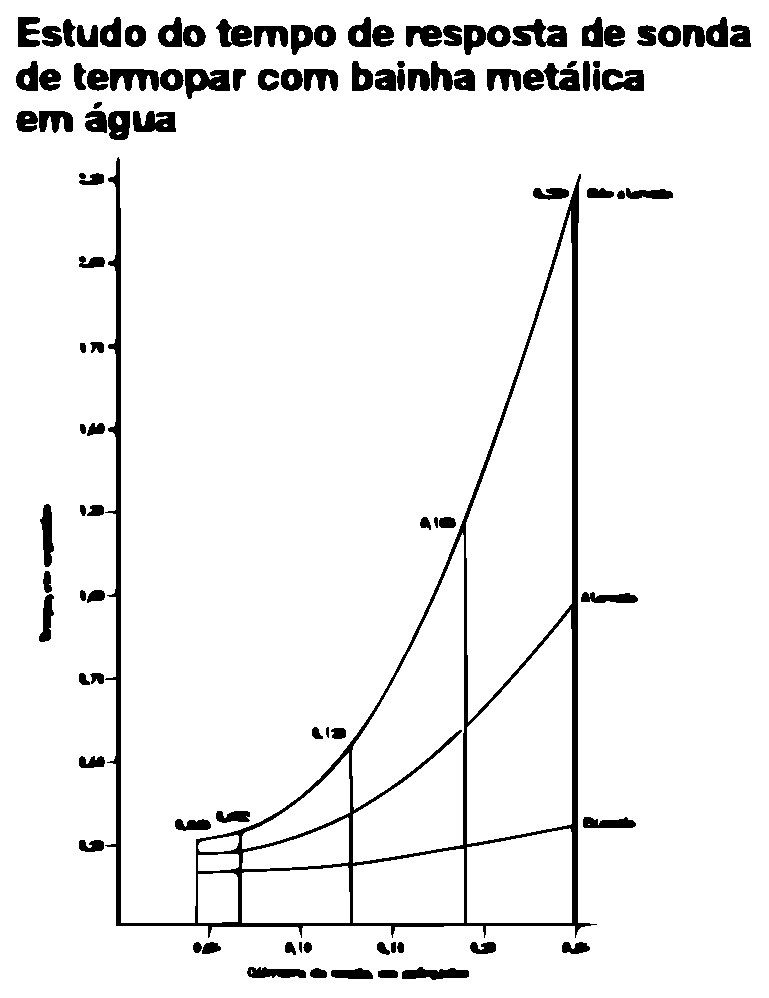
\includegraphics[scale=1]{figuras/Figura3.eps}
	\caption{Estudo do Tempo de Resposta}               
\end{figure}	
\begin{itemize}
	\item \textbf{ Sensor de Temperatura para a tubulação e para o reservatório:}
	\begin{itemize}
		\item \textbf{ Modelo:} Sensor de Temperatura DS18B20;
		\item \textbf{ Descrição:} Sensor de temperatura versão à prova de água do sensor DS18B20; 
		\item \textbf{ Material de composição:}
		\begin{itemize}
			\item \textbf{ Ponteira:} aço inoxidável.
		\end{itemize}
		\item \textbf{ Faixa de temperatura:} de $ -55^oC$ até $+125^oC$;
		\item \textbf{ Precisão:} $\pm0,5^oC$ na faixa de $-10^oC a +85^oC$; 
		\item \textbf{ Alimentação:} 5 VDC;
		\item \textbf{ Tempo de resposta:} menor que 750 ms;
		\item \textbf{ Dimensões:}
		\begin{itemize}
			\item Ponteira com 6 mm de diâmetro por 50 mm de comprimento;
			\item Possui cabo de ligação revestido em PVC de 90 cm;
		\end{itemize}
		\item \textbf{ Comunicação:}
		\begin{itemize}
			\item Possui três fios de interface: Fio Vermelho (VCC), Branco ou Amarelo (DADOS), Preto (GND);
			\item Resolução configurável pelo usuário de 9-bits a 12-bits;
		\end{itemize}
		
		\item \textbf{ Preço:} R\$ 16,80.
\end{itemize}
\end{itemize}
\begin{figure}[!htb]                   
	\centering                          
	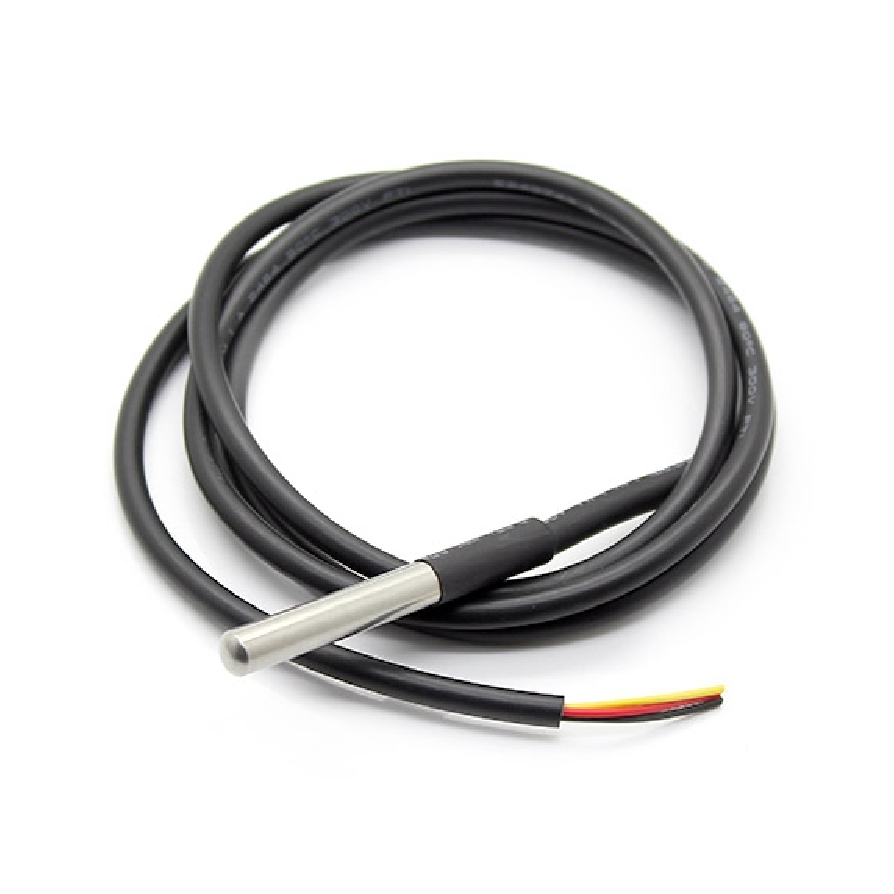
\includegraphics[scale=0.5]{figuras/Figura4.eps}
	\caption{Sensor de Temperatura para a tubulação e para o reservatório}               
\end{figure}
\subsection{Explicação}
Serão utilizados dois sensores deste tipo, um para o reservatório e outro para a tubulação. O sensor que vai no reservatório tem a finalidade de medir a temperatura no local, que segundo estudos do grupo de Transmissão de Calor, deverá estar na faixa de $25 à 30^o$C. A utilização desse sensor é vista como medida de redundância, onde sua principal função é a verificação do funcionamento do sistema de arrefecimento. \\
Já o outro sensor, se encontra próximo a tubulação de saída do sensor de pressão da Kistler, com a finalidade de monitorar a temperatura da água na tubulação. Com as simulações do grupo de Transmissão de Calor foi definido que a temperatura do líquido na tubulação de saída será por volta de $90^oC$. Considerando o local onde o sensor será instalado, será necessário o uso de adaptadores como o bucim, para que possa fixar o sensor na conexão em T adequada. Sendo assim, o uso deste sensor é considerado mais vantajoso, visto que as dimensões do diâmetro e comprimento da bainha especificados (6mm e 30mm, respectivamente) são convenientes para fazer a conexão sem que atrapalhe a medição da temperatura da água na tubulação.\\
Outros fatores cruciais para a escolha desse sensor para essas duas áreas foram a faixa de medição (que é compatível com as duas localidades), o fato do sensor ser à prova d’água e seu tempo de resposta de menos de 750 ms, que geram um ótimo custo-benefício levando em conta que o custo do sensor é mínimo.
\begin{itemize}
	\item \textbf{Sensor de Pressão para a tubulação
	Modelo:} MPX 2200 GP
	\item \textbf{Descrição:} Sensor de Pressão modelo MPX 2200 GP 
	\item \textbf{Tipo de medição:} Tipo Gauge, Pressão de calibre;
	\item \textbf{Pressão de Operação:} 0 a 200 kPa ou 0 a 2 Bar;
	\item \textbf{Temperatura de Operação:} -40 a 125º C;
	\item \textbf{Tempo de resposta:} 1 ms;
	\item \textbf{Tensão de saída:} 40 mV;
	\item \textbf {Alimentação:} 10 a 16 V – 6mA;
	\item \textbf{Sensibilidade:} 0,2 mV/kPa;
	\item \textbf{Dimensões:}
	\begin{itemize}
		\item \textbf{Porta de saída:} Tipo fêmea de 4.62 a 4.93 mm;
	\end{itemize}
	
	\item \textbf{Preço:} R\$ 55,00.
	
\end{itemize}
\begin{figure}[!htb]                   
	\centering                          
	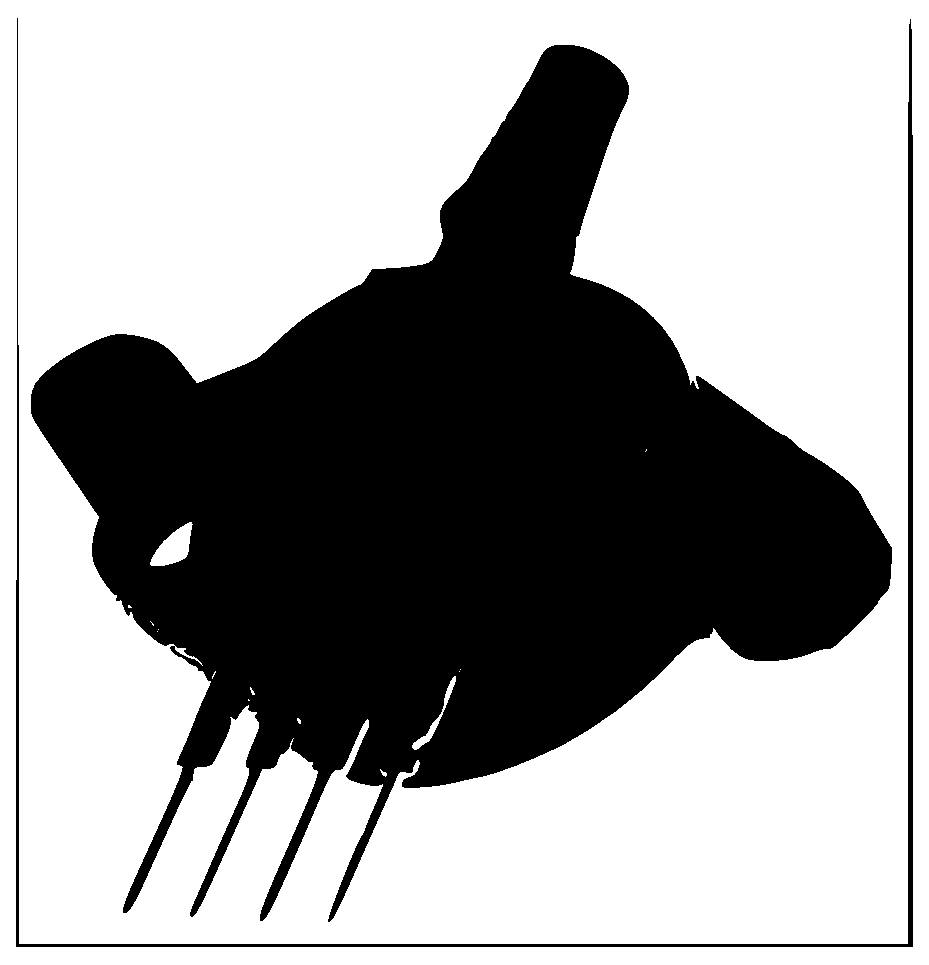
\includegraphics[scale=0.5]{figuras/Figura-5.eps}
	\caption{Sensor de Pressão para a tubulação}               
\end{figure}
